% abtex2-modelo-artigo.tex, v-1.9.2 laurocesar
% Copyright 2012-2014 by abnTeX2 group at http://abntex2.googlecode.com/ 
%

% ------------------------------------------------------------------------
% ------------------------------------------------------------------------
% abnTeX2: Modelo de Artigo Acadêmico em conformidade com
% ABNT NBR 6022:2003: Informação e documentação - Artigo em publicação 
% periódica científica impressa - Apresentação
% ------------------------------------------------------------------------
% ------------------------------------------------------------------------

\documentclass[
	% -- opções da classe memoir --
	article,			% indica que é um artigo acadêmico
	11pt,				% tamanho da fonte
	oneside,			% para impressão apenas no verso. Oposto a twoside
	a4paper,			% tamanho do papel. 
	% -- opções da classe abntex2 --
	%chapter=TITLE,		% títulos de capítulos convertidos em letras maiúsculas
	%section=TITLE,		% títulos de seções convertidos em letras maiúsculas
	%subsection=TITLE,	% títulos de subseções convertidos em letras maiúsculas
	%subsubsection=TITLE % títulos de subsubseções convertidos em letras maiúsculas
	% -- opções do pacote babel --
	english,			% idioma adicional para hifenização
	brazil,				% o último idioma é o principal do documento
	sumario=tradicional
	]{abntex2}


% ---
% PACOTES
% ---

% ---
% Pacotes fundamentais 
% ---
\usepackage{lmodern}			% Usa a fonte Latin Modern
\usepackage[T1]{fontenc}		% Selecao de codigos de fonte.
\usepackage[utf8]{inputenc}		% Codificacao do documento (conversão automática dos acentos)
\usepackage{indentfirst}		% Indenta o primeiro parágrafo de cada seção.
\usepackage{nomencl} 			% Lista de simbolos
\usepackage{color}				% Controle das cores
\usepackage{graphicx}			% Inclusão de gráficos
\usepackage{microtype} 			% para melhorias de justificação
% ---
		
% ---
% Pacotes adicionais, usados apenas no âmbito do Modelo Canônico do abnteX2
% ---
\usepackage{lipsum}				% para geração de dummy text
% ---
		
% ---
% Pacotes de citações
% ---
\usepackage[brazilian,hyperpageref]{backref}	 % Paginas com as citações na bibl
\usepackage[alf]{abntex2cite}	% Citações padrão ABNT
% ---

% ---
% Configurações do pacote backref
% Usado sem a opção hyperpageref de backref
\renewcommand{\backrefpagesname}{Citado na(s) página(s):~}
% Texto padrão antes do número das páginas
\renewcommand{\backref}{}
% Define os textos da citação
\renewcommand*{\backrefalt}[4]{
	\ifcase #1 %
		Nenhuma citação no texto.%
	\or
		Citado na página #2.%
	\else
		Citado #1 vezes nas páginas #2.%
	\fi}%
% ---

% ---
% Informações de dados para CAPA e FOLHA DE ROSTO
% ---
\titulo{Instruções Básicas de Como Instalar e Rodar em Ambiente local o TesteFullStackPleno.}
\autor{Esdras Fragoso da Silva Neto\thanks{esdrasfragoso@gmail.com}}
\local{Brasil}
\data{2019}
% ---

% ---
% Configurações de aparência do PDF final

% alterando o aspecto da cor azul
\definecolor{blue}{RGB}{41,5,195}

% informações do PDF
\makeatletter
\hypersetup{
     	%pagebackref=true,
		pdftitle={\@title}, 
		pdfauthor={\@author},
    	pdfsubject={Modelo de artigo científico com abnTeX2},
	    pdfcreator={LaTeX with abnTeX2},
		pdfkeywords={abnt}{latex}{abntex}{abntex2}{atigo científico}, 
		colorlinks=true,       		% false: boxed links; true: colored links
    	linkcolor=blue,          	% color of internal links
    	citecolor=blue,        		% color of links to bibliography
    	filecolor=magenta,      		% color of file links
		urlcolor=blue,
		bookmarksdepth=4
}
\makeatother
% --- 

% ---
% compila o indice
% ---
\makeindex
% ---

% ---
% Altera as margens padrões
% ---
\setlrmarginsandblock{3cm}{3cm}{*}
\setulmarginsandblock{3cm}{3cm}{*}
\checkandfixthelayout
% ---

% --- 
% Espaçamentos entre linhas e parágrafos 
% --- 

% O tamanho do parágrafo é dado por:
\setlength{\parindent}{1.3cm}

% Controle do espaçamento entre um parágrafo e outro:
\setlength{\parskip}{0.2cm}  % tente também \onelineskip

% Espaçamento simples
\SingleSpacing

% ----
% Início do documento
% ----
\begin{document}

% Retira espaço extra obsoleto entre as frases.
\frenchspacing 

% ----------------------------------------------------------
% ELEMENTOS PRÉ-TEXTUAIS
% ----------------------------------------------------------

%---
%
% Se desejar escrever o artigo em duas colunas, descomente a linha abaixo
% e a linha com o texto ``FIM DE ARTIGO EM DUAS COLUNAS''.
% \twocolumn[    		% INICIO DE ARTIGO EM DUAS COLUNAS
%
%---
% página de titulo
\maketitle

% resumo em português
\begin{resumoumacoluna}
 Este documento tem o objetivo de fornecer instruções de como instalar e rodar em ambiente local o TesteFullStackPleno, conforme o requisitado pela empresa Rockbuzz como requisito de admissão na vaga de emprego Desenvolvedor(a) Full Stack. 
 
 \vspace{\onelineskip}
 
 \noindent
 \textbf{Palavras-chaves}: PHP7.2; HTML5; CSS3; JavaScript:ES6; 
\end{resumoumacoluna}

% ]  				% FIM DE ARTIGO EM DUAS COLUNAS
% ---

% ----------------------------------------------------------
% ELEMENTOS TEXTUAIS
% ----------------------------------------------------------
\textual

% ----------------------------------------------------------
% Introdução
% ----------------------------------------------------------
\section*{Introdução}
\addcontentsline{toc}{section}{Introdução}
O teste consistiu em cria uma api restfull com recurso de posts e as ações de listar, adicionar e atualizar baseada no diagrama  da figura~\ref{diagrama}. 

Foi desenvolvida uma interface de autenticação dos usuários, além de uma interface restrita a usuários autenticados com características administrativas com formulário de postagem e edição de conteúdo.  Similarmente foi desenvolvida uma interface com características de um blog para exibir as postagens.  

Todo código do projeto está disponível no repositório do Github \url{https://github.com/fsdrasfragoso/TesteFullStackPleno}, com instruções básicas de como instalar e rodar em ambiente local.



\begin{figure} [h!]
  \centering
    \caption{Diagrama do Banco dados}
  \label{diagrama}
    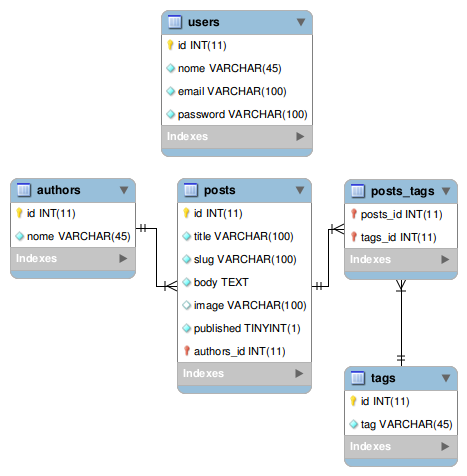
\includegraphics[scale=0.5]{diagra.png}
       
\end{figure}


\footnote{\url{https://github.com/fsdrasfragoso/TesteFullStackPleno}}.



% ----------------------------------------------------------
% Seção de explicações
% ----------------------------------------------------------
\section{Descrição do Código-fonte}

\subsection{DB.class.php}

O arquivo ‘DB.class.php’, é responsável pela conexão com Banco de Dados. Para fazer esta conexão a Class DB utiliza dos recursos do PHP Data Objects - PDO. A utilização do mesmo fornece uma camada de abstração em relação a conexão com o banco de dados visto que o PDO efetua a conexão com diversos bancos de dados da mesma maneira, modificando apenas a sua string de conexão.

O código entre aspas a seguir: "'mysql:host=localhost;dbname=fullstack','root','ecioj’", é a String de conexão a ser modificada para instalar o sistema localmente. Primeiro passo é informar qual o tipo de banco de dados o usuário está utilizando, nesse caso como se pode notar é o Mysql. Em seguida se informa o endereço do servidor do Banco de Dados, que neste cenário é o endereço local.  O passo seguinte é informar o nome do Banco de dados, seguido do usuário e senha que acessaram o servidor.  Mais Abaixo poderá ser notado o código detalhado da Class DB.  

\begin{verbatim}
  class DB{
		private static $conn;
		static function getConn(){
			if(is_null(self::$conn)){
				self::$conn = new PDO('mysql:host=localhost;dbname=fullstack','root','ecioj');
				self::$conn->setAttribute(PDO::ATTR_ERRMODE,PDO::ERRMODE_EXCEPTION);
			}
			return self::$conn;
		}
	}
\end{verbatim}

\subsection{Login.class.php}

A class Login é responsável pela autenticação  dos usuários do sistema, utilizando do conceito de herança ela extends da class DB, herdando a conexão com o Banco de dados e os recursos do PDO. Alterando apenas três constantes é possível fazer a configuração dessa class, permitindo que ela se adeque a qualquer aos mais variados tipos de registro de usuários. As linhas a serem alteradas podem ser vista logo abaixo. 

\begin{verbatim}
  class Login extends DB{
		
		private $tabela = 'users';
		private $prefix = 'fullstack_';
		private $cookie = true;
		public $erro = '';
\end{verbatim}

A constante  \$tabela  é responsável por receber o nome da tabela onde está sendo armazenados os usuários. A \$prefix armazena o prefixo dos cookies de registro de login e login e senha, para salvar no navegador os endereço de email e a senha do usuario. Através desse prefixo é verificado se este um cookie do sistema salvo no navegador permitindo o mesmo lembrar de um ou mais dados de logins.   


\subsection{seguranca.php}

O arquivo seguranca.php é a API de segurança do sistema, ela fornece o serviço de instância de usuários e proteção das páginas.  Quando ela é incluída na página a mesma passa a ser protegida podendo ser acessada somente por usuários logadas no sistema. 

\section{Interface com Caracteristicas de um Blog}

\subsection{index.php}

A página index.php é responsável por exibir todas as postagens dos usuários, deixando-as visível para qualquer um que acessar o endereço da página.  A interface da página como ilustrado pela figura~\ref{index}  tem  características comuns a de um blog. No topo o menu, no centro o conteúdo da página, seguido pelo rodapé. 

\begin{figure} [h!]
  \centering
    \caption{Pagina Index.php}
  \label{index}
    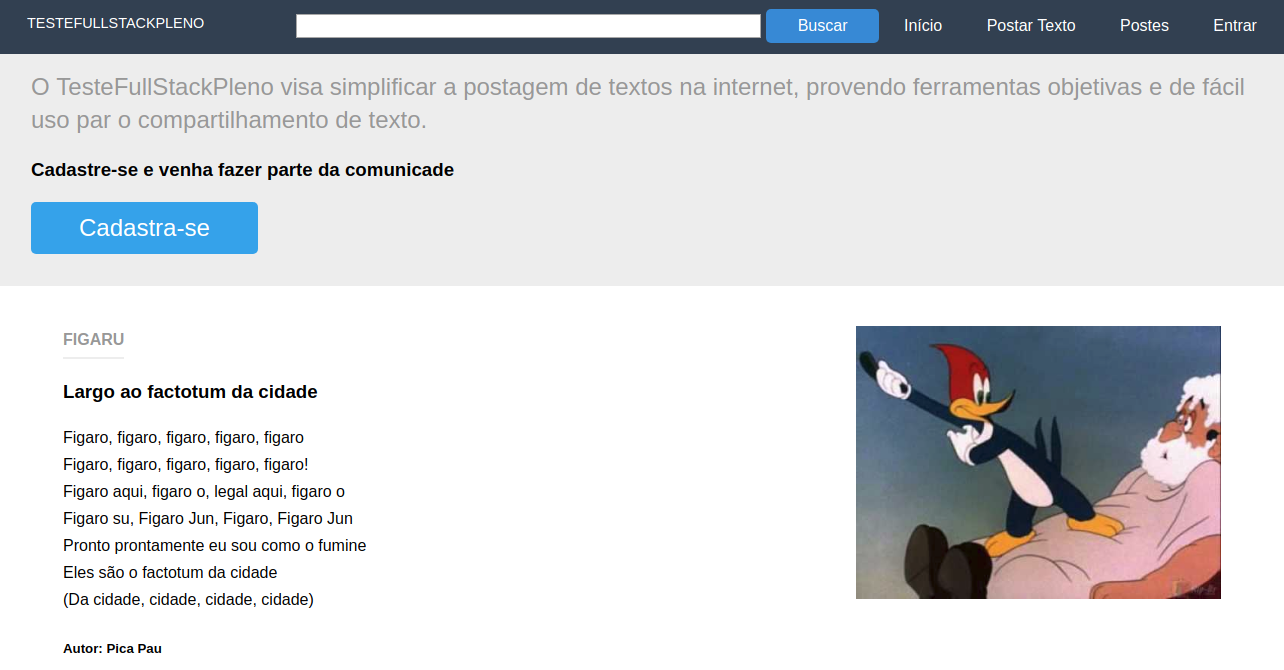
\includegraphics[scale=0.3]{index.png}
       
\end{figure} 


\subsection{buscar.php}

A página buscar.php é responsável exibir os resultados das buscas feitas pelos clientes que do blog.  O resultado é exibido em duas partes primeiro o resultado da busca: pelo nome do autor do texto, título do texto,  slug do texto e corpo do texto. depois é exibido as postagens que possuem tag igual a palavra digitada no formulário de busca.  Essa estrutura é ilustrada pela figura~\ref{buscar}.  

\begin{figure} [h!]
  \centering
    \caption{Página buscar.php}
  \label{buscar}
    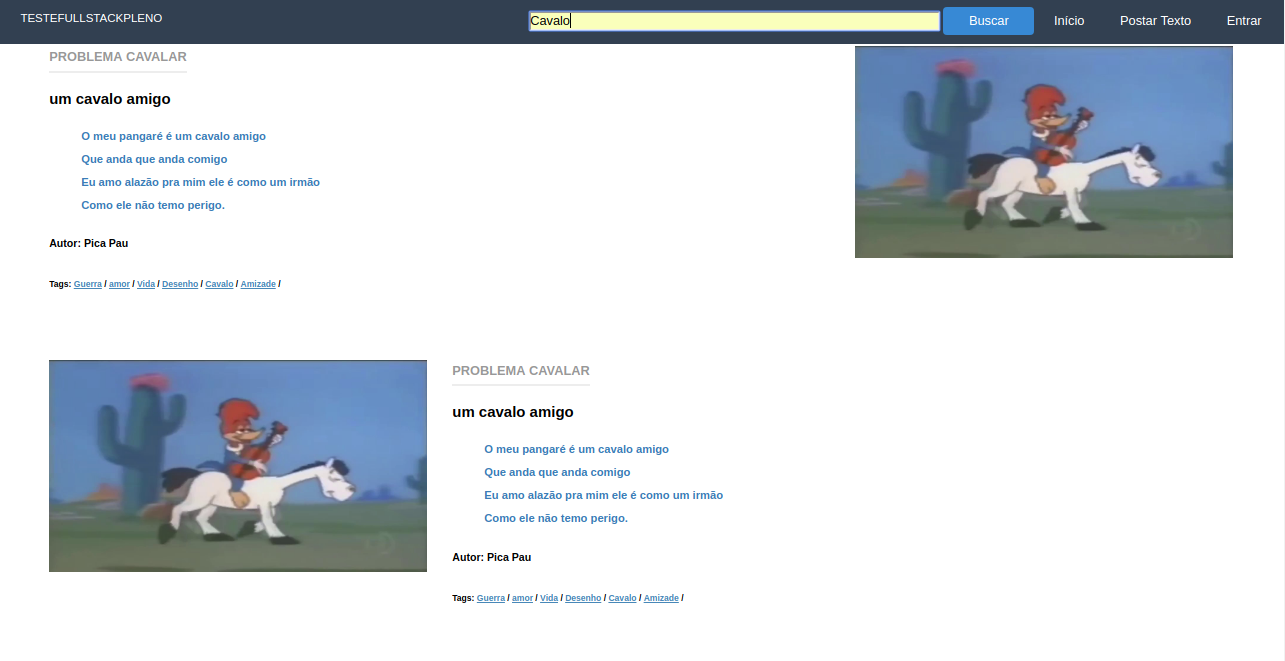
\includegraphics[scale=0.3]{buscar.png}
       
\end{figure} 

\subsection{tag.php} 


A página tag.php lista todos os postes que possuem a tag clicada.  Cada tag exibida nas postagem é também um link que envia via \$\_GET para a página tag.php o id da tag em questão e através do mesmo é feito uma filtragem na tabela posts\_tags  para listar os postes que a possuem. A estrutura de como é feita essa listagem pode ser notado pela figura~\ref{tag}. 


\begin{figure} [h!]
  \centering
    \caption{Página tag.php}
  \label{tag}
    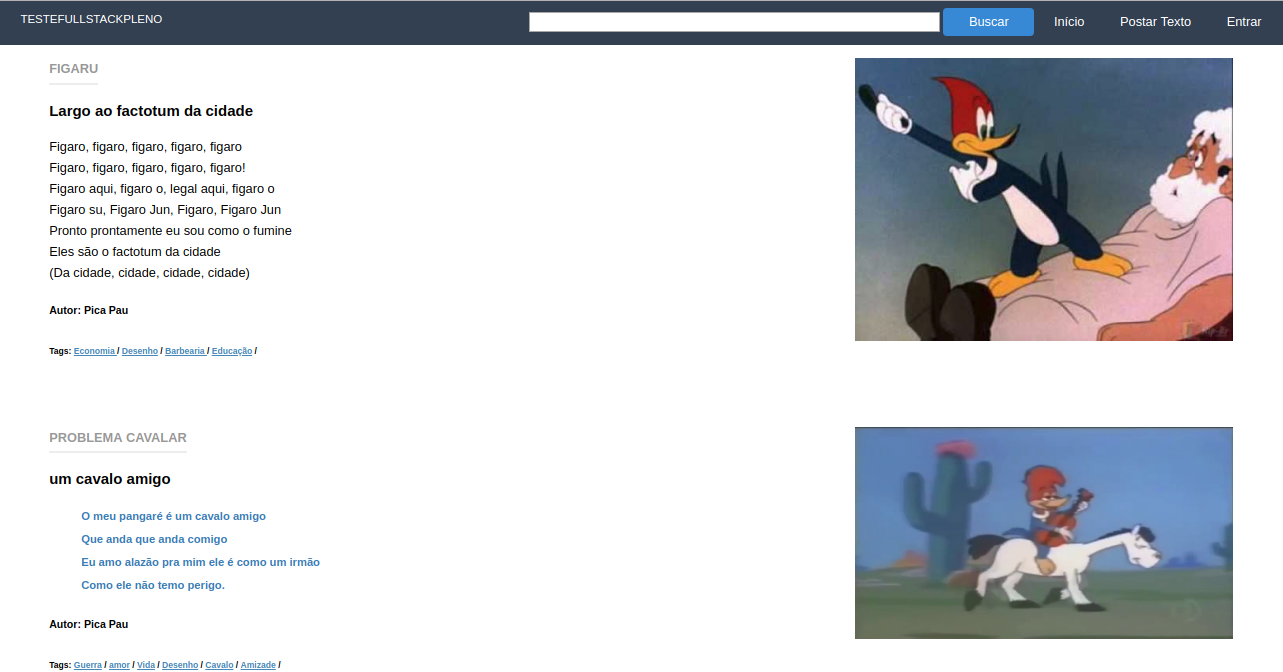
\includegraphics[scale=0.3]{tag.png}
       
\end{figure} 

\begin{verbatim}
 //código responsável por exibir as tags dos posts e gerar os links
  while($tag = $tags->fetch(PDO::FETCH_ASSOC)){
 echo ' <a href="tag.php?id='.$tag['id'].'">'.$tag['tag'].'</a> / '; 
                 }
                 
/*Linha responsável por identificar o ID da tag 
que de ser usada como filtro de listagem dos posts. */

if(isset($_GET['id'])){
            $tag_id = $_GET['id'] ;


\end{verbatim}

\section{Interface Restrita a Usuários Autenticados}

\subsection{editar.php}
A página editar.php aproveita muito do design da página index.php como pode ser notado na figura~\ref{editar}, mas com o diferencial da inclusão dos botões: postar texto, editar e apagar. Onde os usuários devidamente logados podem tanto editar, como apagar e postar textos.  

\begin{figure} [h!]
  \centering
    \caption{Página editar.php}
  \label{editar}
    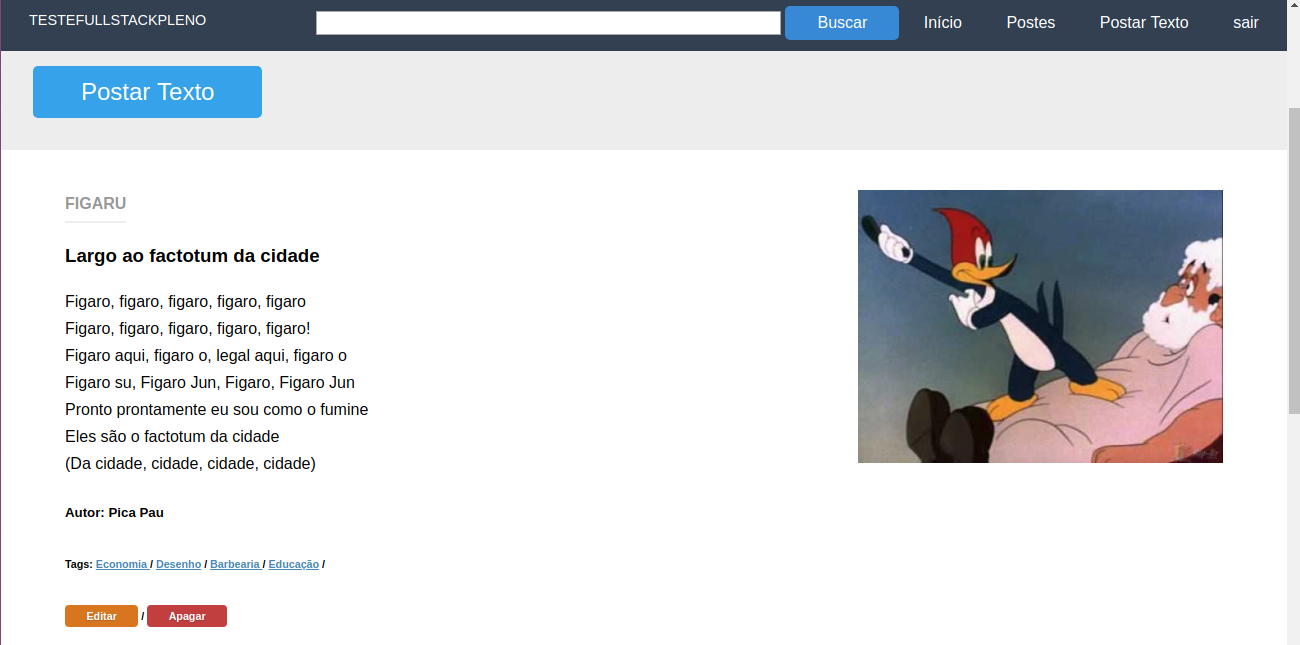
\includegraphics[scale=0.3]{editar.png}
       
\end{figure} 

\section{cadastroPoste.php}

A página cadastroPoste.php é um formulário de cadastro de posts Onde o usuário deve escrever o título, depois o slug, escrever o corpo do texto no ckeditor, selecionar as tagas, caso não exista as tags que necessita basta clicar na opção outra que acionará o javascript e o jequery, que invocará uma API de cadastro de tag, para que a teg seja cadastra e já prontamente selecionada na página. Por fim é selecionado o autor do texto, se não tiver na lista do select basta selecionar a opção outro que novamente o jquery e entra em ação para requisitar uma API de cadastro de autores para já incluir na página o novo autor.  

\begin{figure} [h!]
  \centering
    \caption{Página CadastroPoste.php}
  \label{cadatroPoste}
    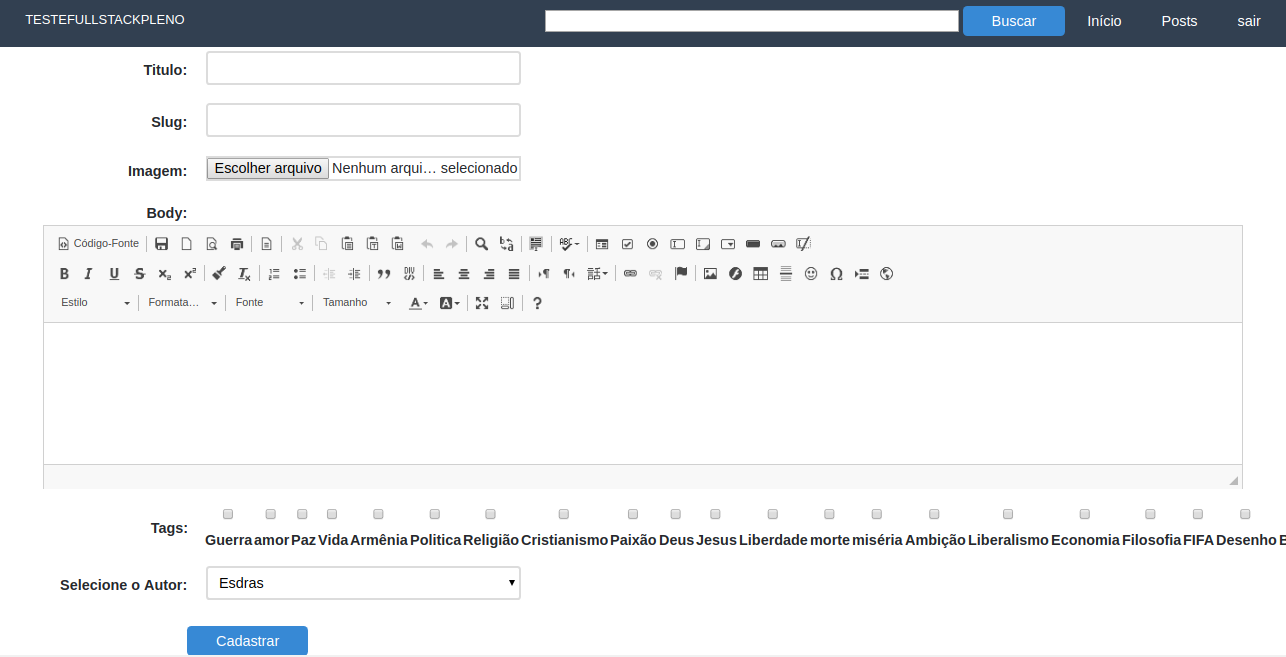
\includegraphics[scale=0.3]{cadastroPoste.png}
       
\end{figure} 

% ---
% Finaliza a parte no bookmark do PDF, para que se inicie o bookmark na raiz
% ---
\bookmarksetup{startatroot}% 
% ---

% ---
% Conclusão
% ---
\section*{Considerações finais}
O Teste foi desenvolvido com boa estrutura e organização, usar bibliotecas específicas e não frameworks full stack's, o código inteligível, escalável, totalmente  versionado do código pelo GIT, possui  filtragem de posts pelas tags, pesquisas internas. O tempo de conclusão foi razoável. Todo  código está disponível no Github pelo link: \url{https://github.com/fsdrasfragoso/TesteFullStackPleno}, e este documento detalha muito mais do que simplesmente instruções básicas de como instalar e rodar em ambiente local. 

Por conta de todos estes fatores apresentados acima é que acredito merecer uma chance de integrar a equipe da Rockbuzz. 


% ----------------------------------------------------------
% ELEMENTOS PÓS-TEXTUAIS
% ----------------------------------------------------------


\end{document}
